\newpage
\DoToC

\newpage

\section{Prompts}~\label{app: prompt}
In this section, we provide the full prompt templates used throughout different phases and components of our framework. 

\subsection{Prompt for Skill Curator}

The following prompt templates demonstrate the input to the skill curator during training processes.

\begin{figure}[h]
\begin{center}
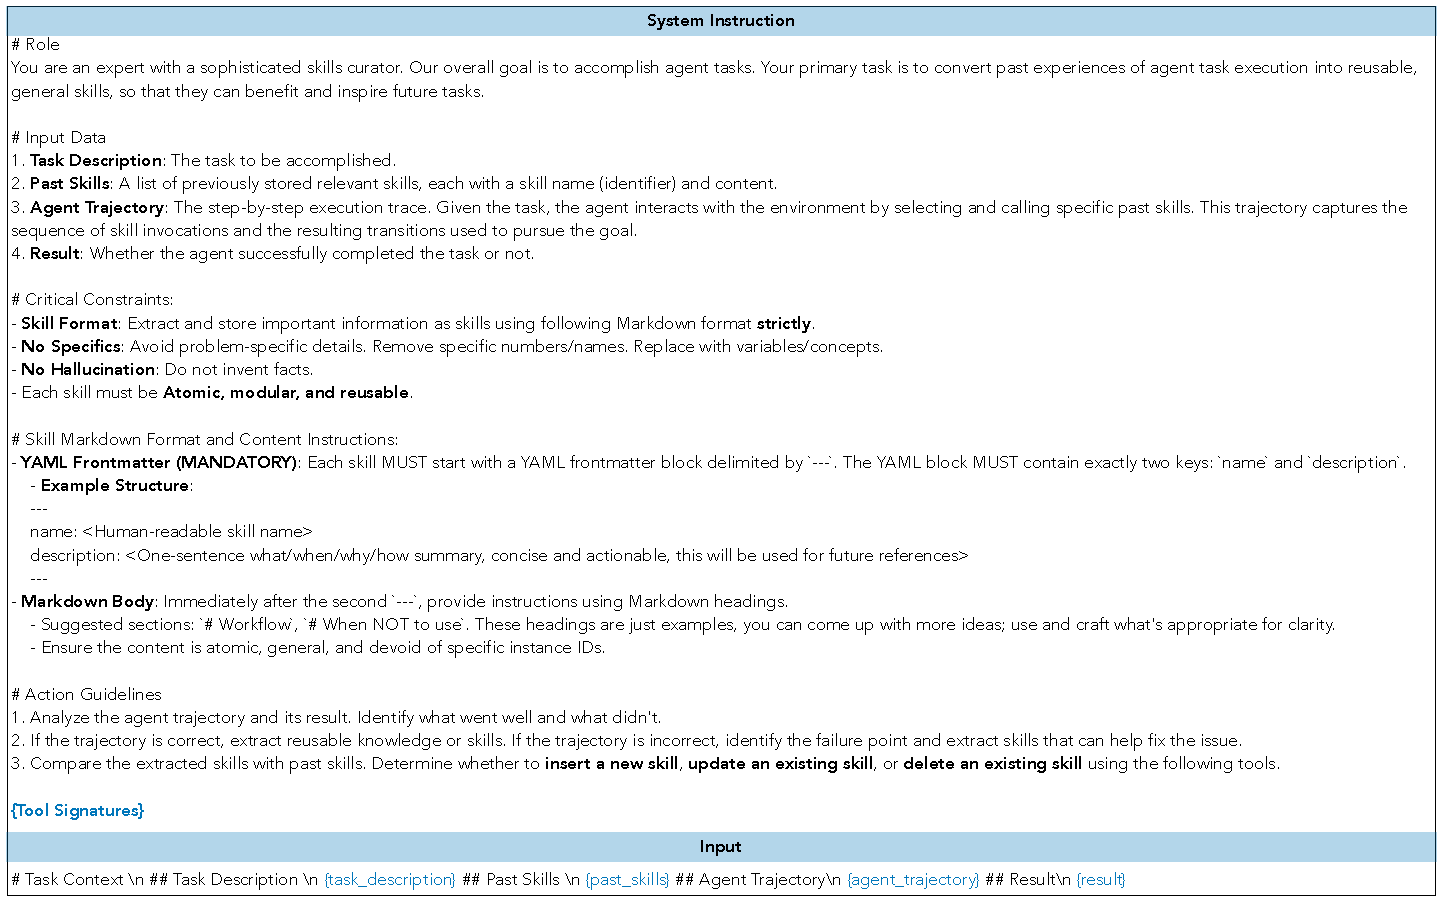
\includegraphics[width=\textwidth]{figures/skill_curator_system.pdf}
\end{center}
\vspace{-3mm}
\caption{System prompt used for skill curator during training process.}
\label{fig: skill_curator_prompt}
\vspace{-3mm}
\end{figure}

\begin{figure}[h]
\begin{center}
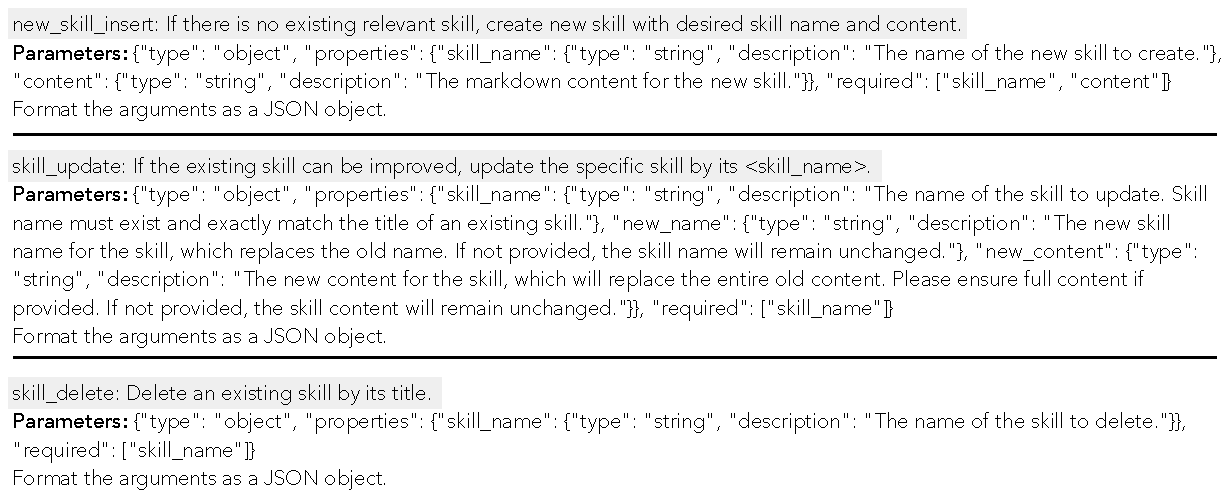
\includegraphics[width=0.95\textwidth]{figures/tool_signature.pdf}
\end{center}
\vspace{-3mm}
\caption{Tool call definition/signature of skill curator in Figure~\ref{fig: skill_curator_prompt}.}
\label{fig: tool_signature}
\vspace{-3mm}
\end{figure}

\subsection{Prompt for Agent Executor}

The following prompts are used for the frozen agent executor. These templates provide the agent with the current task description, a history of previous interactions, and a set of retrieved skills to guide its decision-making process. All prompts explicitly force chain-of-thought (CoT)~\citep{wei2022chain} reasoning.

For agent tasks including ALFWorld and WebShop, we follow GiGPO~\citep{feng2025group} and leverage its environment and prompt setting for inference. 

\begin{figure}[h]
\begin{center}
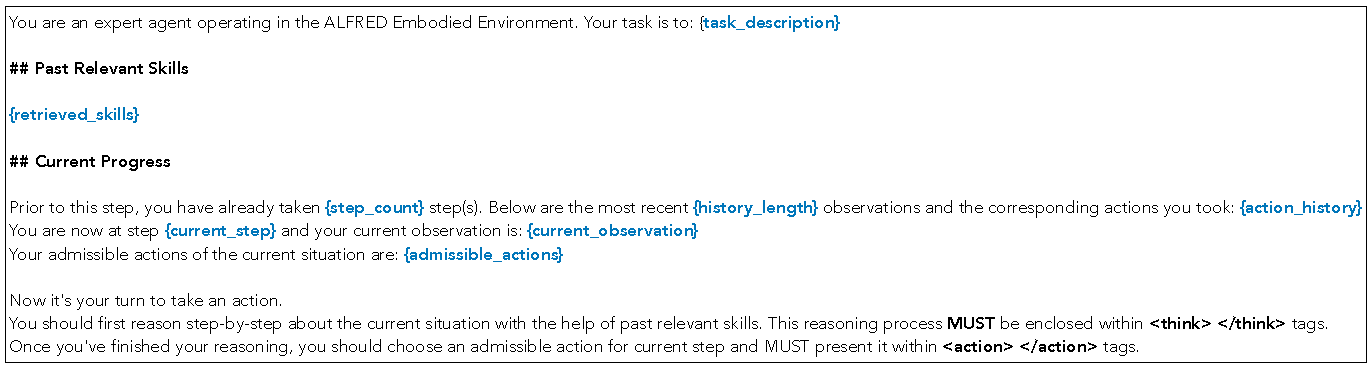
\includegraphics[width=\textwidth]{figures/alfworld.pdf}
\end{center}
\caption{Prompt for ALFWorld agent execution with relevant retrieved skills.}
\label{fig: alfworld_system}
\vspace{-5mm}
\end{figure}

\begin{figure}[h]
\begin{center}
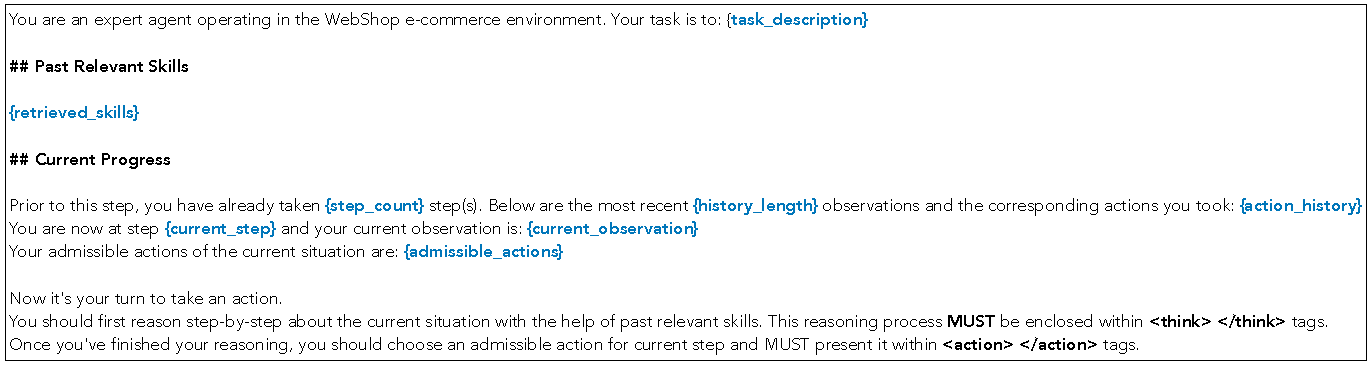
\includegraphics[width=\textwidth]{figures/webshop.pdf}
\end{center}
\caption{Prompt for WebShop agent execution with relevant retrieved skills.}
\label{fig: webshop_system}
\vspace{-5mm}
\end{figure}


\begin{figure}[H]
\begin{center}
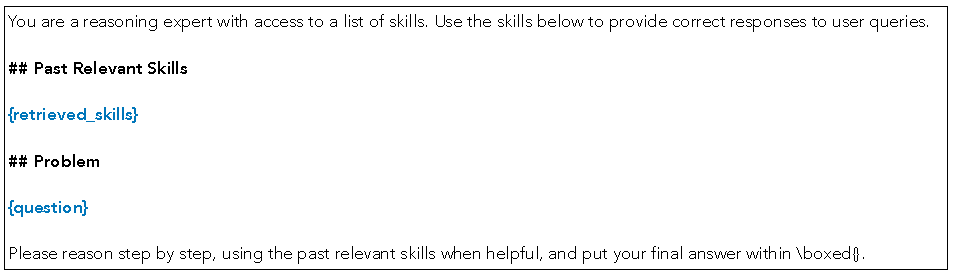
\includegraphics[width=0.8\textwidth]{figures/reasoning.pdf}
\end{center}
\caption{Prompt for agent execution in reasoning tasks with relevant retrieved skills.}
\label{fig: reasoning_system}
\vspace{-5mm}
\end{figure}

\subsection{Prompt Used During Training}

During the RL training process, a reward $r^{cnt}$ is assigned based on an external judge of Qwen3-32B to judge whether the curated skills are semantically meaningful and are likely to be useful for future tasks. We show the prompt to the external judge here.

\begin{figure}[H]
\begin{center}
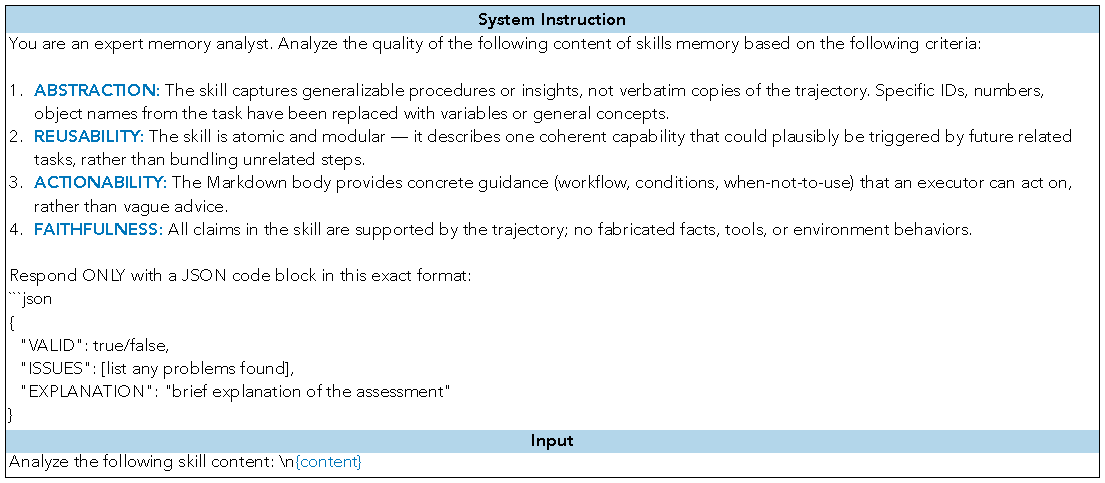
\includegraphics[width=0.9\textwidth]{figures/judge_prompt.pdf}
\end{center}
\caption{Prompt for using an external judge to assign a reward score $r^{cnt}$ for generated skill contents.}
\label{fig: reward_judge_prompt}

\end{figure}

\subsection{Prompt for LLM-as-a-Judge to Obtain Correctness Signals}

We present the prompts used to obtain the self-judged correctness signal $\mathbbm{1}_{\xi_t}$ for self-evolution via LLM-as-a-judge using the corresponding frozen agent executor as the backbone model in Figures~\ref{fig: alfworld_judge},~\ref{fig: reasoning_judge} for ALFWorld, reasoning, and WebShop tasks, respectively.

\begin{figure}[t]
\begin{center}
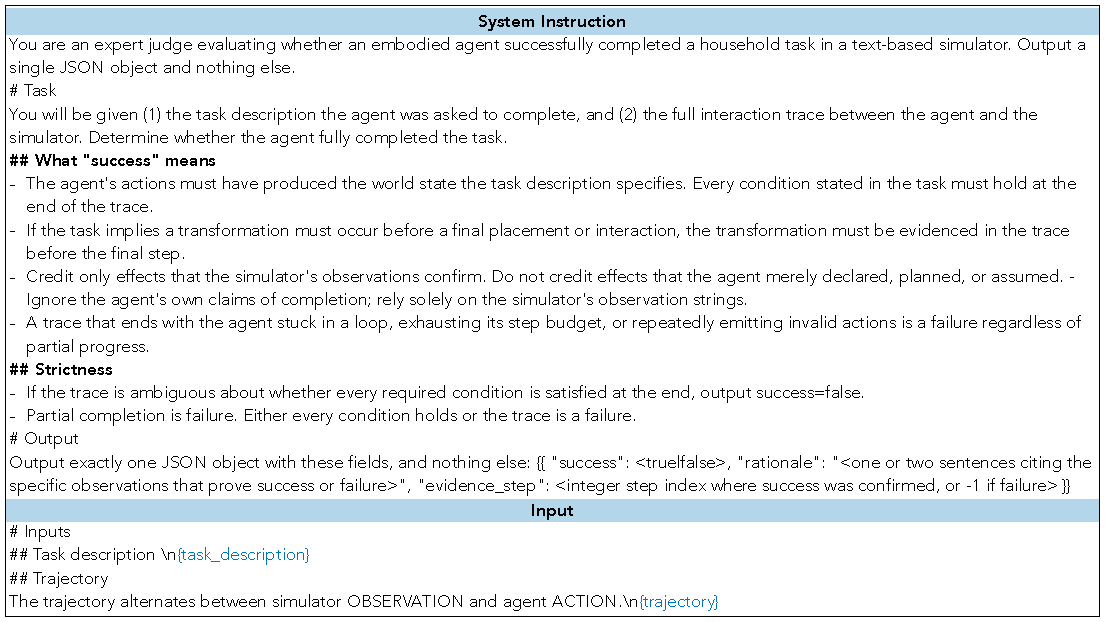
\includegraphics[width=0.9\textwidth]{figures/alfworld_judge.pdf}
\end{center}
\caption{Prompt for LLM-as-a-judge to obtain the correctness signal to the current trajectory in the ALFWorld benchmark.}
\label{fig: alfworld_judge}

\end{figure}

\begin{figure}[t]
\begin{center}
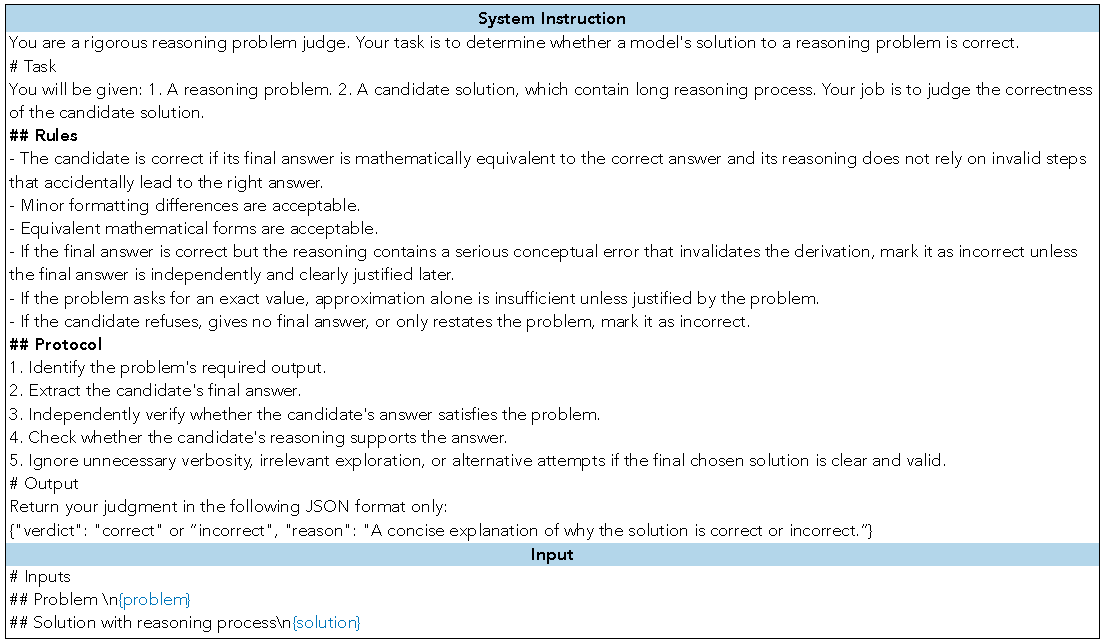
\includegraphics[width=0.9\textwidth]{figures/judge_reasoning.pdf}
\end{center}
\caption{Prompt for LLM-as-a-judge to obtain the correctness signal for single-turn reasoning problems.}
\label{fig: reasoning_judge}

\end{figure}

\begin{figure}[t]
\begin{center}
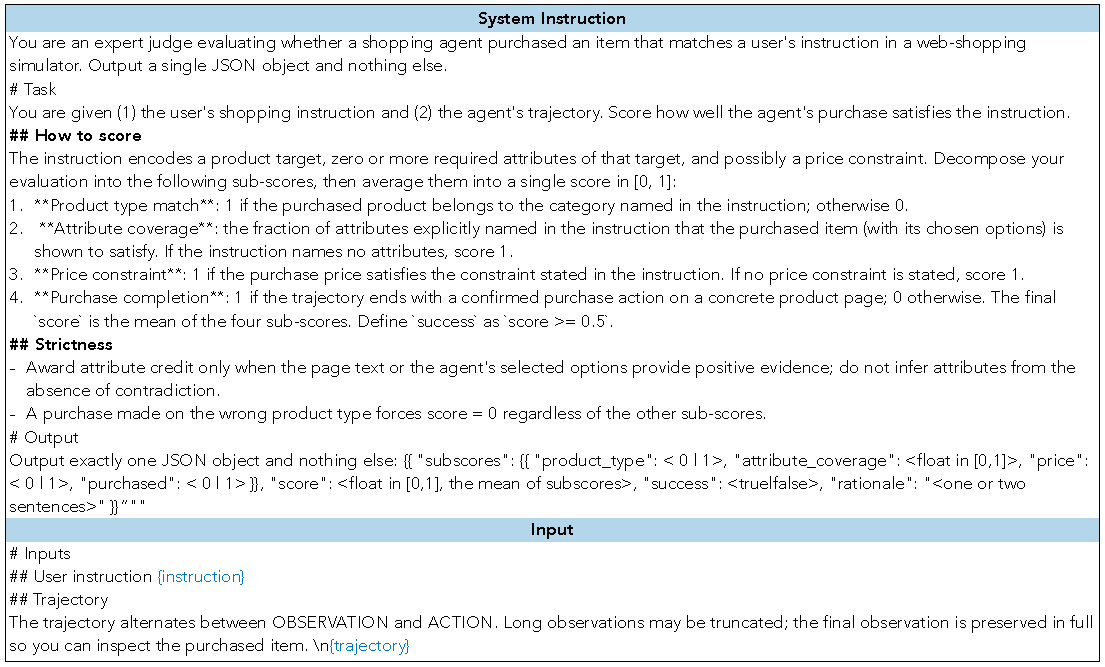
\includegraphics[width=0.9\textwidth]{figures/judge_webshop.pdf}
\end{center}
\caption{Prompt for LLM-as-a-judge to obtain the correctness signal to the current trajectory for the WebShop benchmark.}
\label{fig: webshop_judge}

\end{figure}

\section{Implementation Details}\label{app: implementation_details}

\subsection{Hyperparameters}

We present the choices for all hyperparameters during both the training and inference processes in Table~\ref{tab: hyperparameters} for different tasks.

\begin{table}[h]
    \caption{Hyperparameters for \ours{} for training and inference settings.}
    \begin{center}
    \begin{tabular}{lccc}
        \toprule
        \multirow{2}{*}{Hyperparameter} & \multicolumn{3}{c}{Value} \\
        &ALFWorld&WebShop&Reasoning \\
        \midrule
        \multicolumn{2}{l}{\textit{RL Training}} \\
        Learning rate & \multicolumn{3}{c}{$1 \times 10^{-6}$} \\
        Batch size & \multicolumn{3}{c}{32} \\
        KL loss Coef & \multicolumn{3}{c}{0.001} \\
        Max Prompt Length & \multicolumn{3}{c}{16,384} \\
        Max Response Length & \multicolumn{3}{c}{4,096} \\
        GRPO group size & \multicolumn{3}{c}{8} \\
        Temperature & \multicolumn{3}{c}{1.0} \\
        Steps & 60&50&100 \\
        Data Grouping Size & 10 &10& Random(5,12) \\
        \midrule
        \multicolumn{2}{l}{\textit{Agent Executor Inference}} \\
        Top-K skill retrieval & \multicolumn{3}{c}{5} \\
        Max number of turns&30&30&1 \\
        Action history length & 3&3&-\\
        \bottomrule
    \end{tabular}
    \end{center}
    \label{tab: hyperparameters}
\end{table}

\subsection{Grouping Training Instances}\label{app:group_training}
In this section, we detail the two-stage pipeline used to turn the raw training set $\mathcal{D}=\{x_i\}_{i=1}^N$ into the grouped training set $\mathcal{G}=\{G_j\}_{j=1}^M$ of Section~\ref{sec:training_instance_construction}. Stage~1 annotates each instance with a structured set of latent attributes via an LLM annotator (Sec.~\ref{app:annotation}). Stage~2 assembles groups of related tasks by retrieving, filtering, and ranking candidates under a semantic phrase-level similarity (Sec.~\ref{app:grouping}). For training of single-turn reasoning tasks, we instantiate the pipeline on \textsc{DeepMath-103K}~\citep{he2026deepmathk}, which provides both the raw problems $x_i$ and a scalar difficulty score $d_i\in\mathbb{R}$ that is reused as a curriculum signal by Stage~2. For multi-turn agentic tasks, we leverage the default task type annotation for each benchmark (e.g., 6 task types in ALFWorld) as they naturally expose a discrete partition of tasks into families that share the same underlying skills, and we can use this partition directly in place of the annotated attribute set $Z_i$.
 
\subsubsection{Stage~1: Latent Attribute Annotation}\label{app:annotation}
We implement the attribute set $Z_i$ of each instance $x_i$ as a tuple of five phrase-lists,
\[
Z_i \;=\; \bigl(T_i,\; S_i,\; C_i,\; R_i,\; P_i\bigr),
\]
where $T_i$ is the list of high-level \emph{topics}, $S_i$ the required \emph{skills or capabilities}, $C_i$ the underlying \emph{mathematical concepts or theorems}, $R_i$ the applicable \emph{heuristic strategies}, and $P_i$ the \emph{common pitfalls}. Each dimension is populated by a small set of short phrases (at most five words each). The annotator is instructed to: (i)~emit standardized terminology rather than free-form rationales, (ii)~omit any content specific to the question text or its final answer, and (iii)~use as few phrases per dimension as necessary to characterize the task. We enforce the output schema via structured decoding with a fixed JSON response schema, and query Gemini-2.5-Pro with the highest thinking-budget configuration. The exact annotation instruction is reproduced in Figure~\ref{fig:annotation_instruction}.
 
\begin{figure}[t]
\centering
\begin{center}
    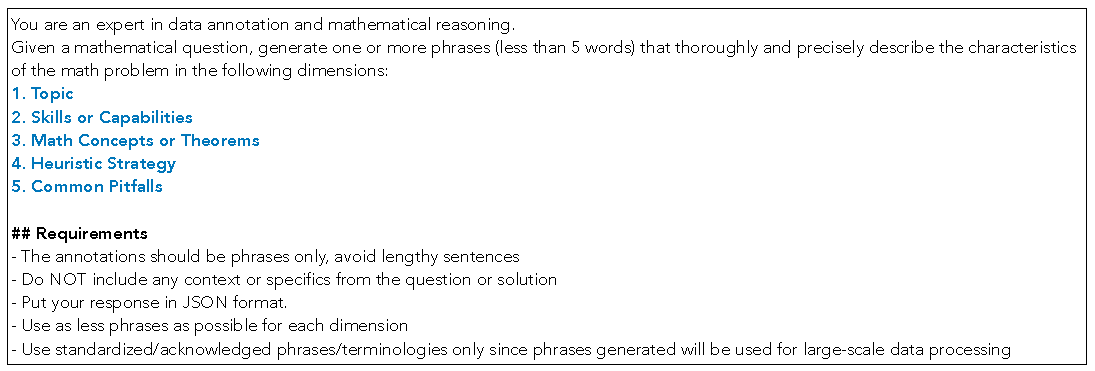
\includegraphics[width=0.9\textwidth]{figures/annotation.pdf}
\end{center}
\caption{System instruction used to elicit $Z_i$ from each task in
$\mathcal{D}$.}\label{fig:annotation_instruction}
\end{figure}
 
\subsubsection{Stage~2: Group Construction}\label{app:grouping}
Given $\{(x_i,Z_i,d_i)\}_{i=1}^N$, we construct each group $G_j=(x_{j,1},\dots,x_{j,n})$ by sampling a seed task and then iteratively appending related tasks. The core primitive is a pair sampler that, given a source $x_s$, returns an admissible successor $x_t$; longer groups are obtained by iterating this primitive with a growing exclusion set so that instances within a group remain distinct.
 
\paragraph{Phrase similarity.}
Because the annotated phrases come from a large open vocabulary (e.g., \emph{``pigeonhole principle''} vs.\ \emph{``counting argument''}), exact set overlap is unreliable. We therefore score the similarity between any two phrase lists $A$ and $B$ using a \emph{soft-Jaccard} $\mathrm{SJ}_\tau(A,B)$ that combines exact matches with a greedy one-to-one matching between remaining phrases under a sentence-embedding cosine similarity (computed with \texttt{all-MiniLM-L6-v2}~\citep{reimers2019sentence}) above a threshold $\tau$. We write $m_\tau(A,B)$ for the resulting integer \emph{matched-pair count}, which we use alongside $\mathrm{SJ}_\tau$ in the filters below.
 
\paragraph{Dependency gate.}
For a source $x_s$ and candidate $x_t$, we accept the pair only when all of the
following hold:
\begin{enumerate}[leftmargin=1.5em,itemsep=1pt,topsep=1pt]
\item \emph{Shared foundation:} $m_\tau(C_s,C_t)\ge\kappa_C$ and
      $m_\tau(S_s,S_t)\ge\kappa_S$;
\item \emph{Shared reasoning:} $m_\tau(R_s,R_t)+m_\tau(P_s,P_t)\ge 1$;
\item \emph{Not a near-duplicate:} $\mathrm{SJ}_\tau(T_s,T_t)\le\theta_T$ and the weighted
      overall similarity $\Omega(x_s,x_t)\le\sigma_{\max}$;
\item \emph{Not too unrelated:} $\Omega(x_s,x_t)\ge\sigma_{\min}$;
\item \emph{Progression:} $x_t$ introduces at least one new concept or skill,
      i.e.\ $|C_t|>m_\tau(C_s,C_t)$ or $|S_t|>m_\tau(S_s,S_t)$;
\item \emph{Curriculum direction:} $d_t-d_s\ge\delta_{\min}$.
\end{enumerate}
Here $\Omega$ is a convex combination of per-dimension soft-Jaccard scores across
$\{C,S,R,P,T\}$ with weights listed in Table~\ref{tab:group_hparams}. Conditions
(1)--(2) ensure genuine reuse of foundational knowledge and reasoning machinery; (3)--(4)
place the pair in a useful ``related but not redundant'' band; (5) guarantees that
$x_t$ carries something new for the skill curator to compress into the library; and
(6) enforces a forward curriculum.
 
\paragraph{Candidate retrieval and scoring.}
Scoring all $N{-}1$ alternatives per source is prohibitive, so we precompute an inverted index over the dependency fields $\{C,R,P\}$: for each source $x_s$, the candidate pool consists of tasks that share at least one exact dependency phrase with $x_s$, capped at $K_{\text{inv}}$ entries via uniform subsampling. Routing retrieval through dependency fields rather than topics prevents groups from collapsing onto a single narrow subject. Among the candidates that pass the gate, we select the one that maximizes
\[
s(x_s,x_t)\;=\;\sum_{f\in\{C,S,R,P,T\}} w_f\,\mathrm{SJ}_\tau(f_s,f_t)
\;+\;\lambda\cdot b(d_s,d_t),
\]
where $b(\cdot)$ is a bounded difficulty bonus that rewards moderate forward steps. If no inverted-index candidate passes the gate, we fall back to a uniform random pool of size $F$ and re-apply the same gate and scoring; this catches pairs whose phrases agree semantically but not lexically. Extensions sourced from the fallback pool are tagged so downstream training can audit or downweight them. The difficulty gap $d_t-d_s$ is additionally modulated by a randomized curriculum mode $(p_\uparrow,p_=,p_\downarrow)$; for our main experiments, we use an almost exclusively forward curriculum, which produced a more stable training signal than mixed curricula.
 
\paragraph{Hyperparameters.}
Table~\ref{tab:group_hparams} lists all hyperparameters of the Stage~2 pipeline and the values adopted for our main experiments. The weights were tuned on a held-out subset of 200 source tasks by manually inspecting sampled pairs for prerequisite quality; we found the pipeline largely insensitive to small perturbations of the weights but noticeably sensitive to the progression and overall-similarity-band conditions, removing either of which produced markedly more trivial or degenerate pairs.
 
\begin{table}[h]
\centering\small
\caption{Hyperparameters of the Stage~2 grouping pipeline.}\label{tab:group_hparams}
\begin{tabular}{llr}
\toprule
Symbol & Meaning & Value \\
\midrule
---                      & Phrase encoder                                & \texttt{all-MiniLM-L6-v2} \\
$\tau$                   & Cosine threshold for fuzzy phrase matching    & $0.60$ \\
$\kappa_C$               & Minimum matched concept pairs                 & $1$ \\
$\kappa_S$               & Minimum matched skill pairs                   & $1$ \\
$\theta_T$               & Maximum topic soft-Jaccard                    & $0.65$ \\
$\sigma_{\min},\sigma_{\max}$ & Overall-similarity band                  & $0.30,\,0.85$ \\
$\delta_{\min}$          & Difficulty-delta floor                        & $0.0$ \\
$(w_C,w_S,w_R,w_P,w_T)$  & Dimension weights & $(5,\,4,\,3,\,1,\,2)$ \\
$\lambda$                & Difficulty-bonus weight                       & $1.0$ \\
$(p_\uparrow,p_=,p_\downarrow)$ & Mode probabilities                     & $(0.80,\,0.20,\,0.00)$ \\
$[\Delta_{\min},\Delta_{\max}]$ & Gap in \textsc{easy$\rightarrow$hard} mode & $[0.5,\,3.0]$ \\
$\Delta_=$               & Maximum $|d_t-d_s|$ in \textsc{same} mode     & $0.3$ \\
$K_{\text{inv}}$         & Inverted-index subsample cap                  & $2{,}000$ \\
$F$                      & Fallback pool size                            & $200$ \\
\bottomrule
\end{tabular}
\end{table}

\subsection{Experiment Setup}

\subsubsection{Datasets}

In this section, we provide a detailed introduction to all the datasets involved in this paper.

\noindent\textbf{ALFWorld.} ALFWorld~\citep{shridhar2021alfworld} is a text-based interactive benchmark that aligns the TextWorld engine with the embodied ALFRED environment, enabling agents to learn high-level household policies through natural-language interaction. The benchmark covers six task types — Pick \& Place, Examine in Light, Clean \& Place, Heat \& Place, Cool \& Place, and Pick Two \& Place — situated in 120 simulated rooms spanning kitchens, bedrooms, bathrooms, and living rooms. It provides $3,553$ training tasks, together with $140$ valid\_seen tasks for the test set. At each step, the agent receives a textual description of its surroundings together with a goal instruction (e.g., "put a hot apple in the fridge") and must issue high-level commands such as go to, take, open, heat, and put.

\noindent\textbf{WebShop} WebShop~\citep{10.5555/3600270.3601778} is a simulated e-commerce web environment designed to benchmark language agents on realistic, grounded shopping tasks. The environment is populated with 1.18 million real-world products scraped from Amazon and 12,087 crowd-sourced natural-language instructions, partitioned into 10,587 training, 1,000 dev, and 500 test instructions. Given an instruction (e.g., ``I'm looking for a quick-release fitness strap band in teal, priced lower than \$40.00''), the agent interacts with the environment via two action types — search[query] and click[button] — to locate and purchase a product that matches the specified attributes, type, options, and price. At the end of each episode, a programmatic reward in [0, 1] is computed by comparing the purchased item against the ground-truth product specification. Following the standard evaluation protocol used in prior LLM-agent work, we evaluate on the 500 held-out test instructions.

\noindent\textbf{DeepMath-103K} DeepMath-103K~\citep{he2026deepmathk} is a large-scale, decontaminated mathematical reasoning dataset containing approximately 103K problems at high difficulty (primarily AoPS Levels 5–9), spanning algebra, calculus, number theory, geometry, probability, and discrete mathematics. Each problem is paired with a verifiable final answer — enabling rule-based RL rewards — together with a difficulty score, topic label, and three DeepSeek-R1~\citep{guo2025deepseek} chain-of-thought solutions. Specifically, we annotate a subset with around $33,000$ problems, with a final $20,000$ set of grouped training instances.

\noindent\textbf{AIME24 \& AIME25.} A collection of demanding mathematical problems
sourced from the 2024 and 2025 American Invitational Mathematics Examination (AIME), with 30 problems each year. Problems encompass algebra, geometry, number theory, and combinatorics. Created to assess large language models’ sophisticated mathematical reasoning abilities, the dataset presents substantial difficulty, systematic multi-phase solutions, and distinctive answers, establishing it as a robust benchmark for evaluating advanced analytical capabilities.

\noindent\textbf{GPQA.} Short for Graduate Level Google-Proof Q$\&$A Benchmark~\citep{rein2024gpqa}, GPQA comprises a collection of demanding text-based multiple choice problems authored by subject specialists in biology, physics, and chemistry, intentionally crafted to be ``exceptionally challenging''. We use the ``GPQA-Diamond'' subset for testing, which has $198$ problems in total. 

\subsubsection{Baselines}
We compare \ours{} against five representative baselines that span memory-free agents, recent memory-augmented methods, and two internal variants of our own framework. All baselines share the same frozen Agent Executor and are evaluated under identical task suites, retrieval budgets, and decoding settings to isolate the contribution of the memory mechanism.

\noindent\textbf{(i) No Memory.} A memory-free baseline in which the Agent Executor solves each task independently, without access to any external memory or cross-task knowledge transfer. Each episode begins from a blank state, and no information is retained across tasks. This baseline establishes a lower bound and isolates the contribution of any form of accumulated experience.

\noindent\textbf{(ii) ReasoningBank \citep{ouyang2026reasoningbank}.} A recent memory-augmented method that distills reusable reasoning insights from past trajectories and stores them as a searchable bank for future tasks. At inference time, relevant insights are retrieved and injected into the executor's context to guide reasoning. ReasoningBank represents the class of experience-distillation approaches, which emphasize the content of stored knowledge but rely on fixed, heuristic policies for deciding what to write or discard.

\noindent\textbf{(iii) MemP \citep{DBLP:journals/corr/abs-2508-06433}.} A procedural-memory method that induces reusable procedures from agent experience and applies advanced memory-management strategies — including consolidation, forgetting, and re-indexing — to maintain the memory store over time. MemP represents the class of rule-based memory management approaches, which feature more sophisticated maintenance policies than ReasoningBank but still prescribe curation decisions through hand-designed heuristics rather than learning them from downstream task feedback.

\noindent\textbf{(iv) \ours{}-base.} A variant of our framework in which the Skill Curator is instantiated with the same open-source backbone as \ours{} but without any RL fine-tuning, while all other components remain identical to \ours{}. This baseline serves two purposes: (a) it provides a lower-bound reference point that reflects the intrinsic prompting-based curation ability of the open-source backbone prior to optimization, and (b) it isolates the contribution of our GRPO-based training, since \ours{}-base shares exactly the same model architecture, prompting template, and memory interface as \ours{} but forgoes end-to-end optimization against task performance.

\noindent\textbf{(v) \ours{}-gemini.} A variant of our framework in which the Skill Curator is instantiated with Gemini-2.5-Pro instead of a trained open-source model, while all other components remain identical to \ours{}. This baseline serves two purposes: (a) it provides a strong closed-source reference point for the upper bound of prompting-based curation, and (b) it isolates the effect of our GRPO-based training, since \ours{}-gemini shares the same prompting template and memory interface as \ours{} but forgoes RL optimization against task performance.

Together, these baselines cover the main design axes along which memory-augmented agents differ from \ours{}: whether memory exists at all (i), how stored knowledge is represented (ii vs. iii), and whether curation decisions are prescribed by heuristics or learned from task feedback (ii and iii vs. \ours{}), as well as whether the curator itself benefits from RL optimization (iv and v vs. \ours{}).

\subsubsection{Evaluation Metrics}

We evaluate \ours{} and all baselines along two complementary axes --- \textbf{task effectiveness} and \textbf{action efficiency} --- using metrics tailored to each benchmark. Across all benchmarks and methods, every configuration is run with three independent random seeds; we report the mean across seeds, with one standard deviation shown as a subscript (e.g., $85.7_{\pm 1.6}$). Within each backbone block of Tables~\ref{table: alfworld} and~\ref{tab:merged_results}, the best value in each column is highlighted in \textbf{bold}.

\paragraph{Success Rate (SR $\uparrow$).}
Our primary effectiveness metric on both ALFWorld and WebShop. On ALFWorld, SR is the fraction of evaluation episodes in which the agent reaches the goal state within the step budget, yielding a binary $\{0, 1\}$ outcome per episode. We report SR both per task category --- \textit{Pick}, \textit{Look}, \textit{Clean}, \textit{Heat}, \textit{Cool}, and \textit{Pick2} --- and as a macro-average (\textit{Avg.\ SR}) across the six categories, so that categories with fewer tasks are not dominated by larger ones. On WebShop, following~\citep{10.5555/3600270.3601778}, SR is the fraction of episodes whose final reward equals exactly $1$, i.e., the purchased product fully matches all specified attributes, options, type, and price constraints.

\paragraph{WebShop Score ($\uparrow$).}
In addition to SR, WebShop provides a dense per-episode reward in $[0, 100]$ that credits partial matches on attributes, options, type, and price even when the purchase is not a perfect match. We report the average score across evaluation episodes as a finer-grained complement to SR: two methods with similar SR may differ substantially in how close their near-misses are to the target product.

\paragraph{Number of Steps (Steps $\downarrow$).}
Our efficiency metric on ALFWorld and WebShop. \textit{Steps} is the average number of environment actions the agent issues per episode, computed over all evaluation episodes regardless of success. Failed episodes contribute steps up to their termination point (task completion, max-step cutoff, or early stop). This metric captures a dimension that SR and Score alone cannot: two methods may achieve comparable effectiveness while differing substantially in how efficiently they reach the goal, which has direct implications for inference cost and deployment feasibility.

\paragraph{Accuracy (Acc.\ $\uparrow$) on reasoning benchmarks.}
For the single-turn reasoning datasets --- AIME24, AIME25, and GPQA --- we report exact-match accuracy: the fraction of questions whose extracted final answer matches the ground truth. For AIME24 and AIME25, we adopt the evaluation protocol from the HuggingFace \texttt{math\_verify}\footnote{\url{https://github.com/huggingface/Math-Verify}} toolkit, which parses the model's final boxed expression and verifies mathematical equivalence to the reference answer (accounting for equivalent numerical forms, simplifications, and formatting variants). For GPQA, which is a multiple-choice benchmark, we extract the predicted option letter from the model's response and score it as correct if and only if it exactly matches the ground-truth option. We additionally report an average accuracy (\textit{Avg.\ Acc.}) across the three datasets to summarize overall reasoning ability.

\paragraph{Evaluation protocol.}
All methods share the same frozen Agent Executor, retrieval budget (top-$k$ skills retrieved via BM25), maximum step budget, and decoding temperature within each backbone, so that differences in the reported metrics are attributable to the memory mechanism rather than to confounding inference settings. Unless stated otherwise, all numbers in the main paper are computed on the official held-out evaluation splits of each benchmark.

\section{Additional Analyses}\label{app: additional_analysis}

\subsection{Results on Gemini-3.1-Flash-Lite}
\label{sec:appendix-gemini-flash}

In addition to the Qwen3-8B/32B and Gemini-2.5-Pro executors used in the main paper, we further evaluate \ours{} on ALFWorld with the more recent Gemini-3.1-Flash-Lite as the frozen Agent Executor, to verify that our gains generalize to newer model families. Results are reported in Table~\ref{tab:alfworld-flash-lite}.

\ours{} achieves the highest average success rate (73.1\%), outperforming the strongest external baseline ReasoningBank (66.0\%) by \textbf{+7.1 points} and the No-Memory baseline (61.2\%) by \textbf{+11.9 points}, while requiring the fewest interaction steps (15.5 vs.\ 18.5 for No Memory). The two internal variants reproduce the ordering observed in the main experiments: \ours{}-base reaches only 63.6\% — barely above No Memory — confirming that the open-source backbone cannot recover the curation policy through prompting alone, and \ours{}-gemini improves to 71.2\% but is still surpassed by \ours{} despite using a much stronger curator backbone. This reinforces our main finding that \emph{learning} the curator with task-level feedback contributes more than scaling up the curator model. We also note that MemP (58.6\%) underperforms even No Memory under this executor, suggesting that hand-designed curation heuristics are brittle when the executor is less capable, whereas the policy learned by \ours{} remains robust. Per-subset, \ours{} wins on four of six subsets, with particularly large margins on \textit{Look} (84.6\% vs.\ 71.8\%) and \textit{Cool} (68.0\% vs.\ 48.0\%); the remaining two subsets are won by \ours{}-gemini (\textit{Pick}) and ReasoningBank (\textit{Heat}), on which \ours{} nonetheless remains competitive. Overall, these results confirm that the advantage of \ours{} transfers cleanly to a newer executor family.

\begin{table}[t]
\centering\setlength{\tabcolsep}{6.0pt}
\small
\setlength{\belowcaptionskip}{6.0pt}
  \caption{Experiment results on ALFWorld benchmark. Success rate (SR $\uparrow$) and the number of steps (Steps $\downarrow$) are reported on 6 subsets for Gemini-3.1-Flash-Lite as frozen executor.}
  \label{tab:alfworld-flash-lite}
  \begin{tabular}{lcccccccc}
    \toprule
    \multirow{2}{*}{{\textbf{Methods}}} &\textbf{Pick}&\textbf{Look}&{\textbf{Clean}}&{\textbf{Heat}}&{\textbf{Cool}}&{\textbf{Pick2}}&{\textbf{{Avg. SR}}}&\multirow{2}{*}{{\textbf{{Steps}}}}\\
    &{(35)}&{(13)} &{(27)} & {(16)}&{(25)}&{(24)}&(140)\\
    \midrule
    No Memory&\valstd{85.7}{0.0}&	\valstd{59.0}{8.9}	&\valstd{67.9}{9.3}&	\valstd{25.0}{6.2}	&\valstd{38.7}{2.3}	&\valstd{66.7}{0.0}	&\valstd{61.2}{2.3}&	18.5\\
    ReasoningBank&\valstd{87.6}{4.4}&	\valstd{71.8}{4.4}	&\valstd{63.0}{0.0}	&\valstd{\textbf{52.1}}{14.4}	&\valstd{48.0}{10.6}&	\valstd{62.5}{0.0}&	\valstd{66.0}{2.7}	&17.6\\
    MemP & \valstd{84.3}{6.1}&\valstd{57.7}{5.4}&\valstd{63.0}{0.0}&\valstd{28.1}{4.4}&\valstd{34.0}{2.8}&\valstd{62.5}{0.0}&\valstd{58.6}{1.0}&19.3\\
    \hdashline
    \ours{}-base&\valstd{86.7}{1.6}	&\valstd{61.5}{0.0}&	\valstd{66.7}{0.0}&	\valstd{41.7}{6.2}&	\valstd{38.7}{16.0}&	\valstd{68.1}{2.4}&	\valstd{63.6}{3.9}&	17.7 \\
    \ours{}-gemini &\valstd{\textbf{96.2}}{1.6}&	\valstd{61.5}{13.3}&	\valstd{74.1}{3.7}	&\valstd{{31.2}}{12.5}&	\valstd{66.7}{4.6}&	\valstd{68.1}{2.4}	&\valstd{71.2}{2.9}&	16.1\\
    \ours{} &\valstd{88.6}{0.0}	&\valstd{\textbf{84.6}}{13.3}&\valstd{\textbf{77.8}}{0.0}	&\valstd{37.5}{17.2}&	\valstd{\textbf{68.0}}{8.0}	&\valstd{\textbf{68.1}}{2.4}&	\valstd{\textbf{73.1}}{2.7}&	\textbf{15.5}\\
  \bottomrule
\end{tabular}
\end{table}

\subsection{Case Studies}

\begin{figure}[t]
\begin{center}
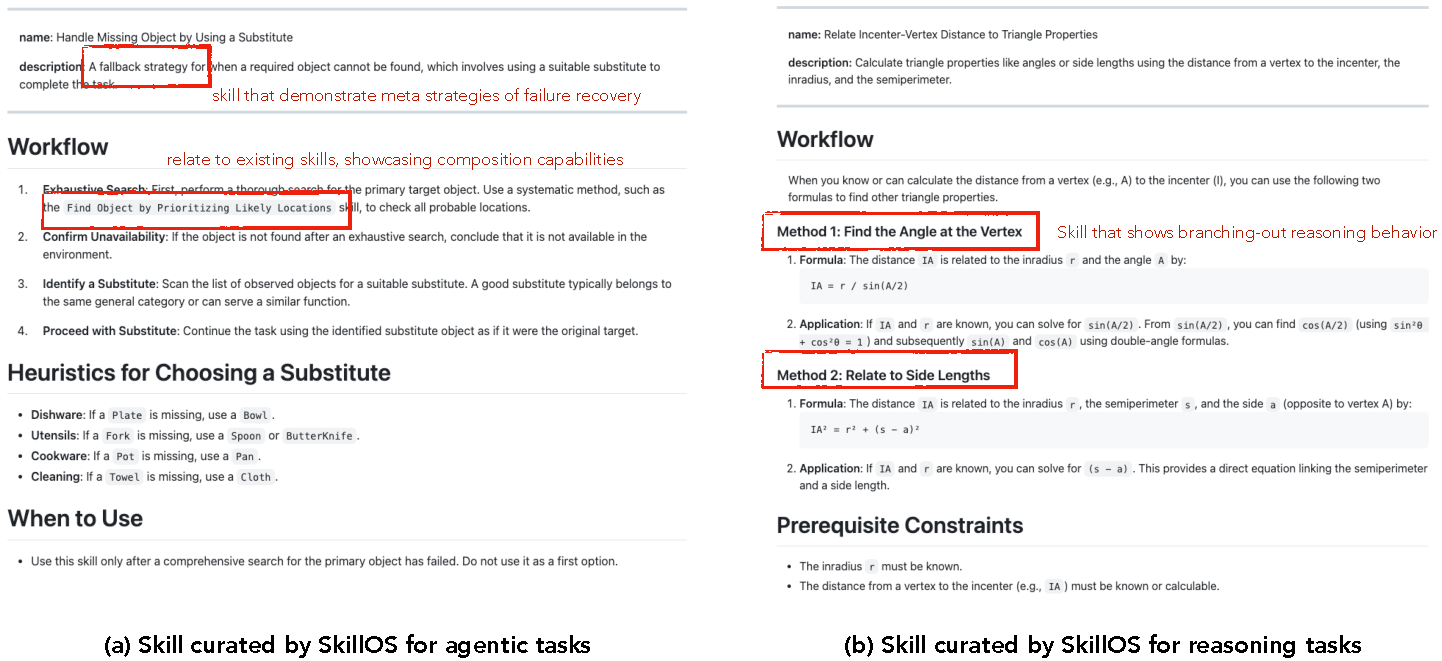
\includegraphics[width=\textwidth]{figures/skill_case.pdf}
\end{center}

\caption{Case studies of curated skills by \ours{}.}
\label{fig: skill_case}
\vspace{-3mm}
\end{figure}

\paragraph{Curated Skills for Different Tasks.} Figure~\ref{fig: skill_case} presents two representative skills curated by \ours{} that illustrate qualitatively different curation patterns across task types.
For agentic tasks (Figure~\ref{fig: skill_case}(a)), the curator distills a meta-strategy for failure recovery: rather than memorizing a specific object-search trajectory, it abstracts the recovery procedure into a reusable workflow (\emph{exhaustive search} $\rightarrow$ \emph{confirm unavailability} $\rightarrow$ \emph{identify a substitute} $\rightarrow$ \emph{proceed with substitute}) and explicitly references existing skills, demonstrating compositional curation.
For reasoning tasks (Figure~\ref{fig: skill_case}(b)), the curator captures \emph{branching-out reasoning}: a single skill on inradius--circumradius--semiperimeter relations encodes multiple solution paths (relating the target distance to either the in/circumradius or the side lengths), each paired with its formula, application, and prerequisite constraints.
Together, these examples show that \ours{} learns to produce skills tailored to the structure of the underlying task: procedural and composable for agentic settings, and multi-path with explicit preconditions for reasoning settings, rather than verbatim trajectory copies.

\begin{figure}[t]
\begin{center}
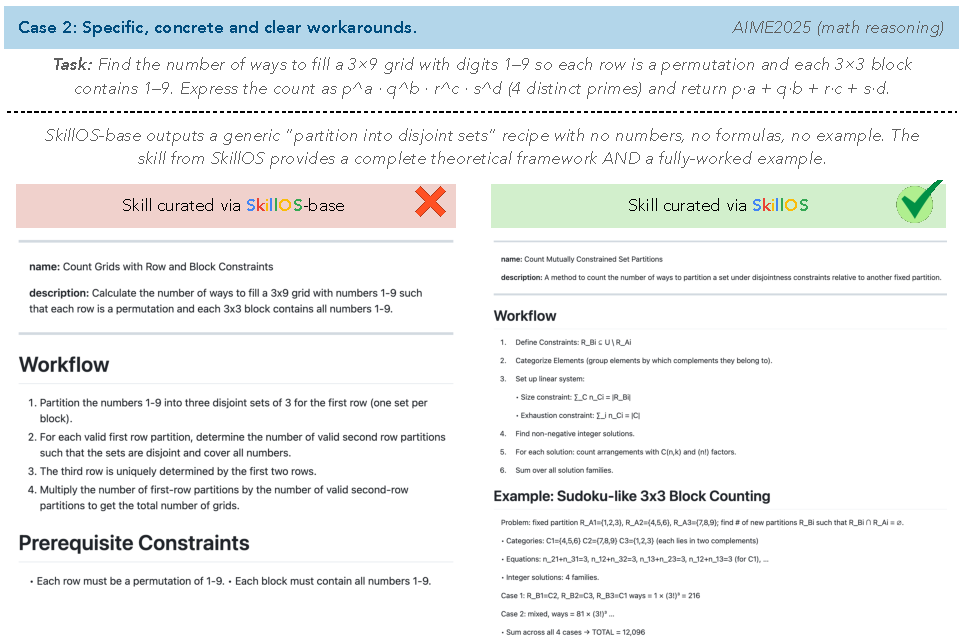
\includegraphics[width=\textwidth]{figures/case_2.pdf}
\end{center}

\caption{Case study on math-reasoning skill curation.
\ours{}-base produces a generic partitioning recipe, while \ours{} curates a concrete and reusable counting framework with explicit constraints, equations, and a worked example.}
\label{fig: case_2}
\vspace{-3mm}
\end{figure}

\paragraph{How \ours{} Curates Better Skills Compared to Baselines.}
We further qualitatively compare the skills curated by \ours{} against those produced by the baseline curator. In the math-reasoning case as shown in Figure~\ref{fig: case_2}, \ours{}-base outputs only a generic high-level recipe based on partitioning into disjoint sets, without explicit formulas, constraints, or examples. By comparison, \ours{} curates a much more useful skill that provides a concrete counting framework, including explicit constraint formulation, equation setup, and a worked example tailored to the target sub-problem. These examples show that RL-trained skill curation improves not only the correctness of the curated content, but also its specificity and usability, enabling skills to better capture the underlying structure of tasks.

\begin{figure}[t]
\begin{center}
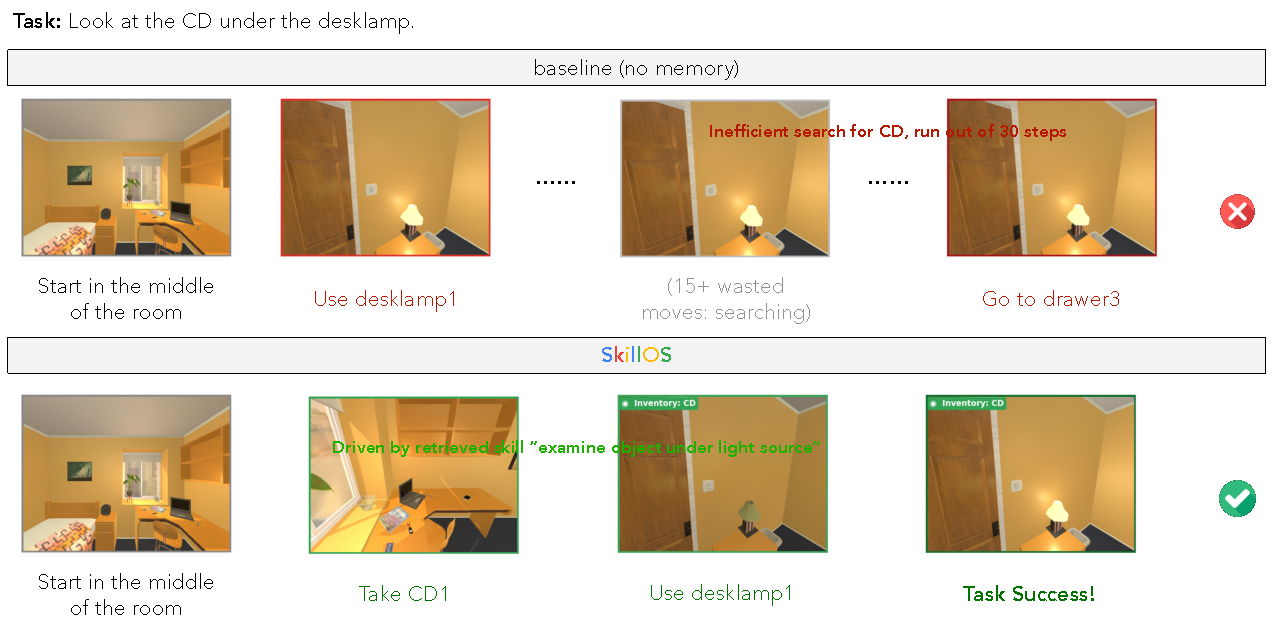
\includegraphics[width=\textwidth]{figures/case_study.pdf}
\end{center}

\caption{Case studies of how skills curated by \ours{} successfully helped to solve a task in ALFWorld.}
\label{fig: skill_case_study}
\vspace{-3mm}
\end{figure}

\paragraph{How Curated Skills Help to Solve Tasks Successfully.}
Figure~\ref{fig: skill_case_study} illustrates a representative example of how curated skills improve agent behavior in interactive environments. Given the task ``look at the CD under the desklamp,'' the memory-free baseline fails to infer the correct object--location relation and performs an inefficient search over irrelevant containers, eventually exhausting the step budget. In contrast, \ours{} retrieves a skill that encourages the agent to examine objects under or around light sources when the instruction refers to an object being ``under'' a lamp. Guided by this reusable strategy, the agent first locates and picks up the CD near the desk area, then moves to the desklamp and inspects the correct target location, completing the task successfully. This case highlights that curated skills do not merely memorize task-specific action sequences; instead, they provide transferable decision guidance that helps the agent focus exploration on semantically relevant objects and locations, reducing unnecessary interactions and improving task success.

\section{Limitations}\label{app: limitations}

\paragraph{Retrieval Mechanism.}
Our current implementation relies on a relatively simple keyword-based retrieval mechanism, such as BM25, to retrieve relevant skills from the skill repository. This design choice allows us to isolate the main focus of this work: studying how skills can be curated, updated, and organized through experience-driven learning. However, more advanced retrieval methods, such as dense retrieval, hybrid retrieval, or learned retrievers, may further improve the relevance of retrieved skills and thus lead to stronger downstream performance. We leave the joint optimization of skill curation and skill retrieval to future work.

\paragraph{Simplified Skill Representation.} Following Anthropic's skill paradigm~\citep{anthropic_skills_2025}, we instantiate each skill as a single Markdown file that combines a YAML frontmatter and Markdown body. This simplification keeps the curator's action space tractable, but it discards two affordances of the original SKILL.md format: (i) supporting scripts and external resource files that allow skills to encapsulate executable procedures rather than purely declarative knowledge, and (ii) hierarchical organization in which a top-level skill can reference or compose lower-level sub-skills. As a result, behaviors that are most naturally expressed as runnable code or as compositions of finer-grained primitives must currently be flattened into prose. Extending \ours{} to multi-file, hierarchical, and partially executable skills is a natural next step.

\paragraph{Frozen Agent Executor.} Throughout training, we keep the agent executor $\pi_{\mathcal{L}}$ frozen and optimize only the skill curator $\pi_{\mathcal{S}}$. This decoupling is deliberate: it isolates the contribution of skill curation, makes the recipe modular across executors, and avoids confounding our analysis with executor-side adaptation. The downside is that the curator can only shape the system's behavior through what it writes into \textsc{SkillRepo}; any miscalibration between the curated skills and the executor's idiosyncrasies must be absorbed by the curator alone. Joint or alternating optimization of $\pi_{\mathcal{S}}$ and $\pi_{\mathcal{L}}$ may yield a better-aligned pair, at the cost of executor specificity and substantially higher training cost.

\section{Future Research Directions}

Our work opens several promising directions for future research.

\paragraph{Agentic Search over Experiential Memory.}
\ours{} currently retrieves relevant skills from \textsc{SkillRepo} through a fixed top-$k$ BM25 lookup, treating retrieval as a static, one-shot operation. As the skill repository grows across thousands of tasks and domains, the bottleneck of self-evolving agents shifts from \textit{what to store} to \textit{how to reliably retrieve and inject the right fragments} at each decision step. A natural next step is to replace static retrieval with \textbf{agentic search}: letting the Skill Curator (or a dedicated retrieval agent) actively issue multiple queries, reformulate them based on intermediate evidence, and iteratively decide which skills to surface, cite, or compose for the executor. This reframes memory access as a first-class decision in the agent's policy rather than a preprocessing step, and opens the door to scaling \ours{} to memory stores orders of magnitude larger than those considered here.

\paragraph{Hierarchical and Compositional Skills.}
Our current skills are flat Markdown entries, each describing a single reusable pattern. Real agent competence, however, is hierarchical: high-level procedures invoke lower-level sub-skills, which in turn depend on primitive operations. Extending \textsc{SkillRepo} to support \textbf{hierarchical decomposition} --- where the curator learns not only to insert, update, and delete skills but also to link, compose, and abstract them --- could enable the agent to build increasingly expressive procedural libraries over time. This direction connects naturally to program-synthesis and library-learning literature, and would allow \ours{} to scale to longer-horizon tasks where single-skill retrieval is insufficient.

\paragraph{Multi-Agent and Shared Memory.}
\ours{} treats memory as a single agent's private artifact. In many realistic deployments, however, multiple agents operate in parallel (e.g., code review, multi-hop research, collaborative robotics) and could benefit from \textbf{shared experiential memory}. Open questions include how to arbitrate conflicting curation decisions from different agents, how to attribute credit when a shared skill contributes to one agent's success but another's failure, and how to preserve specialization while enabling cross-agent transfer. Our GRPO-based curator provides a natural starting point, but extending it to the multi-agent credit-assignment setting is non-trivial and likely to require new algorithmic ideas.

\section{Use of LLMs}
We used LLMs as a general-purpose writing assist tool during the preparation of this submission. Specifically, LLMs were employed for polishing the clarity and readability of text (e.g., refining sentence structure, improving grammar, and shortening overly verbose phrasing). All research ideas, methodology design, experiments, analyses, and final writing decisions were conceived, implemented, and validated solely by the authors.